\section{Random Vectors in High Dimensions}
This chapter mainly deals with the curse of dimensionality, and how vectors interact in these 
high-dimensional settings.



% ----------3.1----------
\subsection{Concentration of the Norm}
\begin{theorem}[Concentration of the norm]
\label{thm:3.1.1}
Let $X = (X_1, \dots, X_n) \in \mathbb{R}^n$ be a random vector with independent, subgaussian coordinates 
$X_i$ satisfying $\mathbb{E}[X_i^2] = 1$. Then 
\[ \left\lVert \lVert x \rVert_2 - \sqrt{n} \right\rVert_{\psi_2} \leq CK^2 \]
where $K = \max_{i} \lVert X_i \rVert_{\psi_2}$ and $C$ is an absolute constant.
\end{theorem}

\begin{proof}
Using \cref{prop:2.6.6}, we can rewrite the above as 
\[ P(\lVert X \rVert_2 - \sqrt{2} \geq t) \leq 2\exp{\left( -\frac{ct^2}{K^4} \right)} \text{ for all } 
t \geq 0. \]
We can prove the bound using Bernstein inequality. If we consider the quantity 
\[ \frac{1}{n}\lVert X \rVert_{2}^2 - 1 = \frac{1}{n}\sum_{i = 1}^{n} (X_i^2 - 1), \]
the above is a sum of independent, mean zero random variables. Moreover, since $XX_i$ are subgaussian, 
$X_i^2 - 1$ are subexponential. Then by the centering lemma (\cref{lem:2.7.8}), we have that 
\[ \lVert X_i^2 - 1 \rVert_{\psi_1} \leq C \lVert X_i^2 \rVert_{\psi_1} 
= C \lVert X_i \rVert_{\psi_2} \leq CK^2. \]
Applying Bernstein inequality ($N = n$ and $a_i = 1/n$), we get that for any $u \geq 0$, 
\begin{align*}
	P \left( \left| \frac{1}{n}\lVert X \rVert_{2}^2 - 1 \right| \geq u \right) 
	&\leq 2\exp{\left[ -c_1 \min_{} \left( \frac{u^2 n}{K^4}, \frac{un}{K^2} \right) \right]} \\
	&\leq 2 \exp{\left[ -\frac{cn}{K^4} \min_{}(u^2, u) \right]}.
\end{align*}
where in the last step, we used the fact that $K$ is bounded below by an absolute constant, since 
\[ 1 = \lVert X_1 \rVert_{L^2} \leq C \lVert X_1 \rVert_{\psi_2} \leq CK \text{ by } \cref{prop:2.6.6}. \]

We'll now use the concentration inequality for $\lVert X \rVert_{2}^2$ to deduce one for 
$\lVert X \rVert_{2}$. We'll use the following propery for all $z, \delta \geq 0$: 
\[ |z - 1| \geq \delta \implies |z^2 - 1| \geq \max_{}(\delta, \delta^2). \]
This is because since $z \geq 0$, $|z + 1| = z + 1 \geq 1$ and $|z + 1| \geq |z - 1|$. Therefore 
\begin{align*}
	|z^2 - 1| 
	&= |z - 1||z + 1| \\
	&\geq |z - 1| \max_{}(|z - 1|, 1) \\
	&\geq \max_{}(\delta, \delta^2).
\end{align*}
Then for any $\delta \geq 0$, 
\begin{align*}
	P \left( \left| \frac{1}{\sqrt{n}} \lVert X \rVert_{2} - 1 \right|  \geq \delta \right) 
	&\leq P \left( \left| \frac{1}{n} \lVert X \rVert_{2}^2 - 1 \right| \geq \max_{}(\delta, \delta^2) \right) \\
	&\leq 2\exp{\left( -\frac{cn}{K^4} \delta^2 \right)}.
\end{align*}
Changing variables with $t = \delta \sqrt{n}$ gives the subgaussian tail.
\end{proof}

\begin{remark}[Thin shell phenomenon]
\label{rmk:3.1.2}
The theorem above shows that random vectors in $\mathbb{R}^n$ mostly stay in a shell of constant thickness 
around the sphere of radius $\sqrt{n}$. This might seem surprising, but here's an intuitive explanation: 

The square of the norm, $\lVert X \rVert_{2}^2$, has a chi-squared distribution with $n$ degrees of freedom. 
Hence its mean is $n$, and standard deviation $\sqrt{2n}$. Thus it makes sense for $\lVert X \rVert_{2}$ 
to deviate by $O(1)$ around $\sqrt{n}$ because 
\[ \sqrt{n \pm P(\sqrt{n})} = \sqrt{n} \pm O(1). \]
\end{remark}



% ----------3.2----------
\subsection{Covariance Matrices and PCA}
The \underline{covariance matrix} of a random vector $X$ taking values in $\mathbb{R}^n$ is 
\[ \mathrm{Cov}(X) = \mathbb{E}[(X - \mu)(X - \mu)^T] = \mathbb{E}[XX^T] - \mu \mu^T, \ \mu = \mathbb{E}[X]. \]
The \underline{second moment matrix} of $X$ is
\[ \Sigma(X) = \mathbb{E}[XX^T]. \]
By translation, the covariance and the second moment matrices are the same, hence many problems can first 
be reduced into the mean zero case.

\subsubsection{Learning from the Covariance Matrix}
The covariance matrix can tell us much more than just the covariance of $X$'s coordinates: 
\begin{proposition}[]
\label{prop:3.2.1}
Let $X$ be a random vector in $\mathbb{R}^n$ with second moment matrix $\Sigma = \mathbb{E}[XX^T]$. Then 
\begin{enumerate}
	\item (1D marginals) For any fixed vector $v \in \mathbb{R}^n$, 
	\[ \mathbb{E}[\left\langle X, v \right\rangle^2] = v^T \Sigma v. \]
	\item (Norm) $\mathbb{E}[\lVert X \rVert_{2}^2] = \mathrm{tr}(\Sigma).$
	\item If $Y$ is an independent copy of $X$, then 
	\[ \mathbb{E}[\left\langle X, Y \right\rangle^2] = \lVert \Sigma \rVert_{F}^2. \]
\end{enumerate}
\end{proposition}

\begin{proof}
(a) Using the linearity of expectation, 
\[ \mathbb{E}[\left\langle X, v \right\rangle^2] = \mathbb{E}[v^T XX^T v]
= v^T \mathbb{E}[XX^T] v = v^T \Sigma v. \]
(b) The diagonal entries of the second moment matrix are $\Sigma_{ii} = \mathbb{E}[X_{ii}^2]$. Then 
\[ \mathbb{E}[\lVert X \rVert_{2}^2] = \mathbb{E}\left[ \sum_{i = 1}^{n} X_i^2 \right] 
= \sum_{i = 1}^{n}\mathbb{E}[X_i^2] = \sum_{i = 1}^{n} \Sigma_{ii}. \]
(c) Since the trace of a matrix is a linear operator, it can be swapped with the expectation: 
\begin{align*}
	\mathbb{E}[\left\langle X, v \right\rangle^2] 
	&= \mathbb{E}[X^T YY^T X] \\
	&= \mathbb{E}[\mathrm{tr}(X^T YY^T X)] \\
	&= \mathbb{E}[\mathrm{tr}(YY^T XX^T)] \\
	&= \mathrm{tr}(\mathbb{E}[X^T X Y^T Y]) \\
	&= \mathrm{tr}(\mathbb{E}[X^T X] \mathbb{E}[Y^T Y]) \\
	&= \mathrm{tr}(\Sigma^2) \\
	&= \lVert \Sigma \rVert_{F}^2.
\end{align*}
\end{proof}


\subsubsection{Principle Component Analysis}
Since the covariance matrix $\Sigma$ is symmetric, it has a spectral decomposition: 
\[ \Sigma = \sum_{i = 1}^{n} \lambda_i v_i v_i^T. \]
Here $\lambda_i$ are the real eigenvalues, and $v_i$ are the corresponding random vectors. There is a nice 
interpretation for eigenvalues from an optimization perspective: 

\begin{proposition}[]
\label{prop:3.2.2}
Let $\Sigma$ be an $n \times n$ symmetric matrix with eigenvalues $\lambda_1 \geq \cdots \geq \lambda_n$ 
and corresponding unit eigenvectors $v_1, \dots, v_n$. Then for every $k = 1, \dots, n$, we have 
\[ \lambda_k = \max_{v \perp \{v_1, \dots, v_{k - 1}\}, \lVert v \rVert_{2} = 1} v^T \Sigma v. \]
\end{proposition}

\begin{proof}
Consider any unit vector $v \in \mathbb{R}^n$ that is orthogonal to $\{v_1, \dots, v_{k - 1}\}$. Using 
the spectral decomposition, we get 
\begin{align*}
	v^T \Sigma v 
	&= v^T \left( \sum_{i = 1}^{n} \lambda_i v_i v_i^T \right) \\
	&= \sum_{i = 1}^{n} \lambda_i (v^T v_i)(v_i^T v) \\
	&= \sum_{i = k}^{n} \lambda_i \left\langle v, v_i \right\rangle^2 \quad \text{(Orthogonality)} \\
	&\leq \lambda_k \sum_{i = k}^{n} \left\langle v, v_i \right\rangle^2 \\
	&\leq \lambda_k.
\end{align*}
We also have that $v_k^T \Sigma v_k = v_k^T (\lambda_k v_k) = \lambda_k$, which reaches the minimal value, 
hence the proof is complete.
\end{proof}

Therefore we have the following corollary: 
\begin{corollary}[PCA]
\label{cor:3.2.3}
Let $X$ be a random vector in $\mathbb{R}^n$ whose covariance matrix has eigenvalues $\lambda_1 \geq \cdots 
\geq \lambda_n \geq 0$ and eigenvectors $v_1, \dots, v_n$. Then 
\[ \lambda_k = \max_{v \perp \{v_1, \dots, v_{k - 1}, \lVert v \rVert_{2} = 1} 
\mathrm{Var}(\left\langle X, v \right\rangle). \]
The maximum is attained at $v_k$.
\end{corollary}	

For a random vector $X \in \mathbb{R}^n$ representing data, 
the top eigenvector of the covariance matrix gives the first \textit{principle component}, indicating the 
direction with has the largest spread, with $\lambda_1$ as the variance in that direction.

\begin{remark}[Dimensionality reduction]
\label{rmk:3.2.4}
It often happens with real data that only a few eigenvalues are large and informative, while the rest are 
small and treated as noise. Therefore even if the data comes in high-dimensionsal, it is basically 
low-dimensional hence you just have to project onto the lower dimensional subspace to perform PCA.
\end{remark}


\subsubsection{Isotropic Distributions}
\begin{definition}[]
\label{def:3.2.5}
A random vector $X$ in $\mathbb{R}^n$ is called \underline{isotropic} if 
\[ \mathbb{E}[XX^T] = I_n \]
where $I_n$ denotes the identity matrix in $\mathbb{R}^n$.
\end{definition}

\cref{prop:3.2.1} implies that $X$ is isotropic if and only if 
\[ \mathbb{E}[\left\langle X, v \right\rangle^2] = \lVert v \rVert_{2}^2 \text{ for any fixed 
vector } v \in \mathbb{R}^n. \]
The above implies that isotropic distributions spread equally in all directions, because the RHS of the 
equation does not depend on the direction of $v$.

\begin{note}[Standardizing]
In one dimension, a random variable $X$ can be standardized to a zero mean, unit variance random variable 
$Z$ by doing 
\[ Z = \frac{X - \mu}{\sqrt{\mathrm{Var}(X)}} \implies X = \mu + \mathrm{Var}(X)^{1/2}Z. \]
This is also true in higher dimensions: 
\[ Z = \mathrm{Cov}(X)^{-1/2}(X - \mu) \implies X = \mu + \mathrm{Cov}(X)^{1/2}Z. \]
Moreover, the idea still holds even if the covariance matrix is not invertible (Exercise 3.10)!
\end{note}



% ----------3.3----------
\subsection{Examples of High-dimensional Distributions}


\subsubsection{Standard Normal}
A random vector $Z$ has the \underline{standard normal distribution in $\mathbb{R}^n$} if its coordinates 
are independent standard normal variables. Its density is 
\[ f_Z(z) = \frac{1}{(2 \pi)^{n/2}} e^{-\lVert z \rVert_{2}^2 / 2}, z \in \mathbb{R}^n. \]

The standard normal distribution is isotropic. Moreover, it is \textit{rotation-invariant}:

\begin{proposition}[Rotation invariance]
\label{prop:3.3.1}
Consider a random vector $Z \sim N(0, I_n)$ and a fixed orthogonal matrix $U$. Then 
\[ UZ \sim N(0, I_n). \]
\end{proposition}

In particular, by looking at the first coordinate of $UZ$, we get 
\[ (UZ)_1 = \left\langle U_1, Z \right\rangle \simN(0, 1) \]
where $U_1$ is the first row of $U$. Since this is an arbitrary unit vector, all 1D marginals of the 
multivariate standard normal distribution are $N(0, 1)$. More generally: 

\begin{corollary}[1D marginals of the standard normal distribution]
\label{cor:3.3.2}
Consider $Z \sim N(0, I_n)$ and any fixed $v \in \mathbb{R}^n$. Then 
\[ \left\langle Z, v \right\rangle \sim N(0, \lVert v \rVert_{2}^2). \]
\end{corollary}

From the above, we get 
\begin{corollary}[Sum of independent normals is normal]
\label{cor:3.3.3}
Consider independent normal random variables $X_i \sim N(\mu_i, \sigma_i^2)$. Then, 
\[ \sum_{i = 1}^{n} X_i \sim N(\mu, \sigma^2), \ \mu = \sum_{i = 1}^{n}\mu_i, 
\sigma^2 = \sum_{i = 1}^{n} \sigma_i^2. \]
\end{corollary}

\begin{proof}
We can write $X_i = \mu_i + \sigma_i Z_i$, where $Z_i$ are independent standard normal random variables. 
Then 
\[ \sum_{i = 1}^{n} X_i = \mu + \sum_{i = 1}^{n} \sigma_i Z_i = \mu + 
\left\langle Z, v \right\rangle \text{ where } v = (\sigma_1, \dots, \sigma_n). \]
Then by \cref{cor:3.3.3}, $\left\langle Z, v \right\rangle \sim N(0, \sigma^2)$ hence 
\[ \mu + \left\langle Z, v \right\rangle \sim N(\mu, \sigma^2). \]
\end{proof}


\subsubsection{General Normal}
\begin{definition}[]
\label{def:3.3.4}
A random vector $X$ in $\mathbb{R}^n$ is \underline{normally distribute} if it can be obtained via an 
affine transformation of a standard normal random vector $Z \sim I(0, I_k)$, i.e.
\[ X = \mu + AZ, \ \mu \in \mathbb{R}^n, \ A \in \mathbb{R}^{n \times k}. \]
Here $X$ has mean $\mu$ and covariance matrix $\Sigma = AA^T$.
\end{definition}

\begin{proposition}[Uniqueness of normal]
\label{prop:3.3.5}
The distribution of $X$ is uniquely determined by $\mu$ and $\Sigma$. Specifically, $X$ has the same 
distribution as 
\[ Y = \mu + \Sigma^{1/2}Z', \ \Sigma = AA^T, \ Z' \sim N(0, I_n). \]
\end{proposition}

\begin{proof}
We'll use a version of the \textit{Cramer-Wold device}, which says that the distributions of all 1D marginals 
uniquely determine the distribution in $\mathbb{R}^n$. This means if $X, Y$ are random vectors in $\mathbb{R}^n$ 
and $\left\langle X, u \right\rangle$ and $\left\langle Y, u \right\rangle$ have the same distribution for all 
$u \in \mathbb{R}^n$, then $X$ and $Y$ have the same distribution.

We check that $AZ$ and $\Sigma^{1/2} Z'$ have the same distribution: 
\[ \left\langle AZ, v \right\rangle = \left\langle Z, A^T v \right\rangle \sim N(0, 
\lVert A^T v \rVert_{2}^2), \text{ and } \left\langle \Sigma^{1/2}Z', v \right\rangle 
\sim N(0, \lVert \Sigma^{1/2} v \rVert_{2}^2). \]
From the above, $\lVert A^T v \rVert_{2}^2 = \lVert \Sigma^{1/2} v \rVert_{2}^2$ since $\Sigma = AA^T$. 
Therefore the proof is complete.
\end{proof}

If $\Sigma$ is invertible, the density has the formula below: 
\begin{proposition}[]
\label{prop:3.3.6}
If $\Sigma$ is invertible, the PDF of a multivariate normal distribution is 
\[ f(x) = \frac{1}{(2 \pi)^{n/2}|\Sigma|^{1/2}} \exp{\left( -\frac{1}{2}(x - \mu)^T \Sigma^{-1} 
(x - \mu)\right)}, x \in \mathbb{R}^n. \]
\end{proposition}

\begin{proof}
Exercise 3.15.
\end{proof}

A special property for normal distributions is that independence and uncorrelation are equivalent, which 
it not true generally: 
\begin{corollary}[Jointly normal random variables]
\label{cor:3.3.7}
Random variables $X_1, \dots, X_n$ are jointly normal if the random vector $X = (X_1, \dots, X_n)$ is 
normally distributed. Jointly normal random variables are independent if and only if they are uncorrelated.
\end{corollary}

\begin{proof}
If $X_i$ are uncorrelated, $\Sigma$ is diagonal. Then the density function can be factored into marginals, 
i.e. 
\[ f(x) = f_1(x) \times \cdots \times f_n(x) \text{ for all } x \in \mathbb{R}^n. \]
The joint density of random variables $X_i$ factors if and only if $X_i$ are independent, hence we're done.
\end{proof}


\subsubsection{Uniform on the Sphere}
\begin{proposition}[A sphere is isotropic]
\label{prop:3.3.8}
The uniform distribution on $S^{n - 1}$ with radius $\sqrt{n}$ is isotropic.
\end{proposition}

\begin{proof}
Let $X \sim \mathrm{Unif}(S^{n - 1})$. By symmetry, for distinct $i, j$, $(X_i, X_j)$ has the same distribution 
as $(-X_i, X_j)$. Therefore 
\[ \mathbb{E}[X_i X_j] = -\mathbb{E}[X_i X_j] \implies \mathbb{E}[X_i X_j] = 0. \]
Moreover, since $\lVert X \rVert_{2} = 1$, 
\[ 1 = \mathbb{E}[\lVert X \rVert_{2}^2] = \mathbb{E}[X_1^2] + \cdots + \mathbb{E}[X_n^2]. \]
The $X_i$ are identically distributed, hence $\mathbb{E}[X_i^2] = 1/n$, hence the coordinates of $\sqrt{n}X$ 
are uncorrelated with second moment equal to 1, hence $\sqrt{n}X$ is isotropic.
\end{proof}

\begin{note}[Isotropic Vectors are almost Orthogonal]
In the high-dimensional world, pick two random points, and they most likely will be orthogonal!

Consider $X, Y \sim \text{Unif}(S^{n - 1})$. Then $\sqrt{n}X, \sqrt{n}Y$ are i.i.d. and isotropic by 
\cref{prop:3.3.8}. By (c) from \cref{prop:3.2.1}, 
\[ \mathbb{E}[\left\langle \sqrt{n}X, \sqrt{n}Y \right\rangle^2] = \mathrm{tr}(I_n) = n. \]
Fividing the above by $n^2$ we obtain 
\[ \mathbb{E}[\left\langle X, Y \right\rangle^2] = \frac{1}{n}. \]
Then applying Markov's inequality, we get 
\[ |\left\langle X, Y \right\rangle| = O(1/ \sqrt{n}) \text{ with high probability}. \]
\end{note}

\begin{note}[Gaussian and spherical distributions are similar]
Both $N(0, I_n)$ and $\mathrm{Unif}(S^{n - 1})$ are isotropic and rotation-invariant. 
\[ g \sim N(0, I_n) \implies \frac{g}{\lVert g \rVert_{2}} \sim \mathrm{Unif}(S^{n - 1}). \]
Informally, we can say that 
\[ N(0, I_n) \approx \mathrm{Unif}(\sqrt{n}S^{n - 1}). \]
This defies the low-dimensional intuition. This is because there is almost no volume near the origin 
in high dimensions. 
\end{note}

To say this in rigorous terms: 
\begin{theorem}[Projective CLT]
\label{thm:3.3.9}
Let $X \sim \mathrm{Unif}(S^{n - 1})$. Then 
\[ \sqrt{n}\left\langle X, v \right\rangle \to N(0, 1) \text{ in distribution as } n \to \infty. \]
In fact, the CDF converges uniformly: 
\[ \sup_{v \in S^{n - 1}} \sup_{t \in \mathbb{R}} |P(\sqrt{n}\left\langle X, v \right\rangle \leq t) 
- P(g_1 \leq t)| \to 0 \]
where $g_1 \sim N(0, 1)$.
\end{theorem}

\begin{proof}
We can assume $X = g / \lVert g \rVert_{2}$ with $g \sim N(0, I_n)$ from above. By rotation invariance, 
the distribution of $\left\langle X, v \right\rangle$ is the same for all $v \in \mathbb{R}^n$. Therefore 
we can choose $v = e_1$ and get 
\[ \left\langle X, e_1 \right\rangle = \frac{g_1}{\lVert g \rVert_{2}}. \]
We'll decompose into a "good event" and a "bad event" that has probability decaying to zero. By the gaussian 
decay tail in \cref{thm:3.1.1},
\[ E_n := \{ |\lVert g \rVert_{2} - \sqrt{n}| \leq \ln{n} \} \text{ is likely: } 
p_n := P(E_n^c) \to 0. \]
If $E_n$ occurs and $t \geq 0$ (which we can assume because of symmetry), then the event of interest 
$\sqrt{n} \left\langle X, e_1 \right\rangle \leq t$ implies 
\[ g_1 \leq \frac{t \lVert g \rVert_{2}}{\sqrt{n}} \leq t \left( 1 + \frac{\ln{n}}{\sqrt{n}} \right) =: t_n. \]
Splitting the event based on whether $E_n$ occurs, we get 
\begin{align*}
	P(\sqrt{n}\left\langle X, v \right\rangle \leq t) 
	&\leq P (\sqrt{n}\left\langle X, v \right\rangle \leq t \text{ and } E_n) + P(E_n^c) \\
	&\leq P(g_1 \leq t_n) + p_n.
\end{align*}
Hence 
\[ P(\sqrt{n}\left\langle X, v \right\rangle \leq t) - P(g_1 \leq t) 
\leq P(g_1 \in [t, t_n]) + p_n. \]
The density of $g_1$ on $[t, t_n]$ is bounded by $e^{-t^2 / 2}$, so 
\[ P(g_1 \in [t, t_n]) + p_n \leq e^{-t^2 / 2}(t_n - t) + p_n 
= e^{-t^2 / 2}t \frac{\ln{n}}{\sqrt{n}} + p_n \leq \frac{C \ln{n}}{\sqrt{n}} + p_n. \]
The RHS does not depend on $v$ or $t$, and goes to zero as $n \to \infty$.

We can also show that $P(g_1 \leq t) - P(\sqrt{n}\left\langle X, v \right\rangle \leq t)$ also goes to 
zero. Combining the two bounds completes the proof.
\end{proof}

\begin{remark}[Density of 1D marginals of the sphere]
\label{rmk:3.3.10}
The density of the 1D marginals of the uniform distribution on the sphre of radius $\sqrt{n}$ can be 
computed. It is in fact proportional to $(1 - x^2 / n)^{\frac{n-3}{2}}$ (Exercise 3.27). For large $n$, 
this approximates $e^{-x^2 / 2}$, which is exactly the Gaussian limit.
\end{remark}


\subsubsection{Uniform on a Convex Set}
Let $K \subset \mathbb{R}^n$ be a convex set. A random variable $X$ is uniformly distributed 
in $K$, denoted $X \sim \mathrm{Unif}(K)$, if its density is $1/\mathrm{Vol}(K)$ on $K$ and zero everywhere 
else.

The mean of $X$ is 
\[ \mu = \mathbb{E}[X] = \frac{1}{\mathrm{Vol}(K)} \int_{K}^{}  \ dx, \]
which is the center of gravity of $K$. If $\Sigma$ is the covaraince matrix of $K$, then the standard score 
$Z := \Sigma^{-1/2}(X - \mu)$ is an isotropic random vector from \cref{def:3.2.5}. In fact, $Z$ is uniformly 
distributed in the affinely transformed copy of $K$: 
\[ Z \sim \mathrm{Unif}\left( \Sigma^{-1/2}(K - \mu) \right). \]
Therefore there is an affine transformation $T$ which makes $T(K)$ isotropic. In convex geometry, we can 
consider $T(K)$ as a well-conditioned version of $K$, which makes algorithms like finding the volume work 
better.


\subsubsection{Frames}
A frame extends the concept of a basis, but drops the requirement of linear independence. Frames are intimately 
connected to discrete isotropic distributions: 
\begin{proposition}[Parseval frames]
\label{prop:3.3.11}
For any vectors $u_1, \dots, u_N$, the following are equivalent: 
\begin{enumerate}[label=(\roman*)]
	\item (Parseval identity) $\lVert x \rVert_{2}^2 = \sum_{i = 1}^{N} \left\langle u_i, x \right\rangle^2$ 
	for each $x \in \mathbb{R}^n$.
	\item (Frame expansion) $x = \sum_{i = 1}^{N} \left\langle u_i, x \right\rangle u_i$ for each $x \in 
	\mathbb{R}^n$.
	\item (Decomposition of identity) $I_n = \sum_{i = 1}^{N} u_i u_i^T$.
	\item (Isotropy) The ranodm vector $X \sim \mathrm{Unif}\{\sqrt{N}u_1, \dots, \sqrt{N}u_N\}$ is isotropic.
\end{enumerate}
A set of vectors satisfying these equivalent properties is called a \underline{Parseval frame}.
\end{proposition}

\begin{proof}
(i) $\Rightarrow$ (iv)
The identity for (i) can be written as 
\[ \lVert x \rVert_{2}^2 = \frac{1}{N} \sum_{i = 1}^{N} \left\langle \sqrt{N} u_i, x \right\rangle^2 
= \mathbb{E}[\left\langle X, x \right\rangle^2]. \]
Since this holds for all $x \in \mathbb{R}^n$, the random vector is isotropic.

(iv) $\Rightarrow$ (iii)
Since $X$ is isotropic, 
\[ I_n = \mathbb{E}[XX^T] = \frac{1}{N}\sum_{i = 1}^{N} \left( \sqrt{N} u_i \right) 
\left( \sqrt{N} u_i \right)^T = \sum_{i = 1}^{N} u_i u_i^T. \]

(iii) $\Rightarrow$ (ii)
Multiply both sides by the vector $x$ gives the result.

(iii) $\Rightarrow$ (ii)
Taking the inner product with the vector $x$ gives the result.
\end{proof}

\begin{example}[Coordinate distribution]
\label{ex:3.3.12}
The standard basis $\{e_1, \dots, e_n\}$ in $\mathbb{R}^n$ is a Parseval frame. Therefore, a coordinate 
random vector 
\[ X \sim \mathrm{Unif}\{\sqrt{n}e_1, \dots, \sqrt{n}e_n\} \]
is isotropic. Among all high-dimensional distributions, Gaussian is often the best to work with and the 
coordinate distribution is the worst.
\end{example}

\begin{example}[Mercedes-Benz frame]
\label{ex:3.3.13}
An example of a Parseval frame that is not linearly independent is the set of $N$ equispaced points on the 
circle of radius $\sqrt{2/N}$, shown below:
\begin{center}
	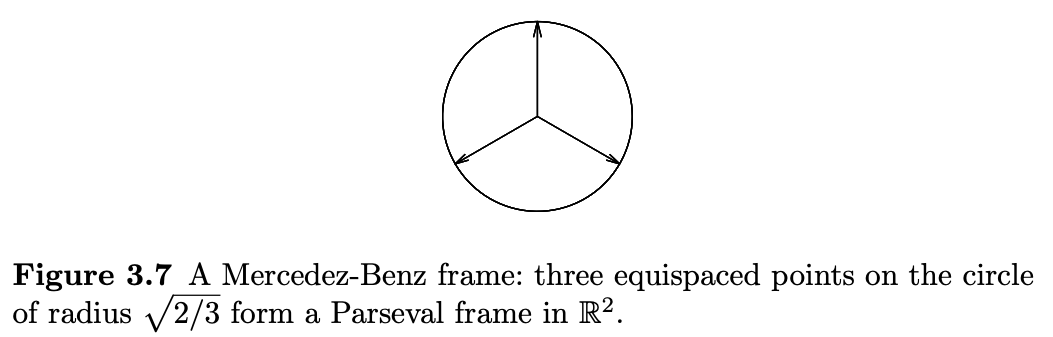
\includegraphics[width=0.8\textwidth]{Chapter 3/fig3-7.png}
\end{center}
\end{example}

Here are two more examples of isotropic distributions:

\begin{example}[Uniform on the discrete cube]
\label{ex:3.3.14}
Let $X$ be a Rademacher random vector, that is, 
\[ X \sim \mnathrm{Unif}(\{-1, 1\}^n). \]
Then $X$ is isotropic.
\end{example}

\begin{example}[Product distributions]
\label{ex:3.3.15}
Any random vector $X = (X_1, \dots, X_n)$ whose coordinates $X_i$ are independent random variables with zero 
mean and unit variance is isotropic. 
\end{example}



% ----------3.4----------
\subsection{Subgaussian Distributions in High Dimensions}
\begin{definition}[]
\label{def:3.4.1}
A random vector $X$ in $\mathbb{R}^n$ is called \underline{subgaussian} if the one-dimensional marginals 
$\left\langle X, v \right\rangle$ are subgaussian random variables for all $v \in \mathbb{R}^n$. 

The \underline{subgaussian norm} of $X$ is defined by taking the maximal subgaussian norm of the marginals 
over all unit vectors: 
\[ \lVert X \rVert_{\psi_2} = \sup_{v \in S^{n - 1}} \lVert \left\langle X, v \right\rangle \rVert_{\psi_2}. \]
\end{definition}

Below are some examples :)

\subsubsection{Gaussian, Rademacher, and More}
\begin{lemma}[Distributions with independent subgaussian coordinates]
\label{lem:3.4.2}
Let $X = (X_1, \dots, X_n)$ be a random vector in $\mathbb{R}^n$ with independent, mean zero, subgassian 
coordinates $X_i$. Then $X$ is a subgaussian random vector, and 
\[ \max_{i \leq n} \lVert X_i \rVert_{\psi_2} \leq \lVert X \rVert_{\psi_2} 
\leq C \max_{i \leq n} \lVert X_i \rVert_{\psi_2}. \]
\end{lemma}

\begin{proof}
The lower bound comes from picking $v$ as a standard basis vector in \cref{def:3.4.1}. 

For the upper bound, fix any $v = (v_1, \dots, v_n) \in S^{n - 1}$. Then 
\begin{align*}
	\lVert \left\langle X, v \right\rangle \rVert_{\psi_2}^2 
	&= \lVert \sum_{i = 1}^{n} v_i X_i \rVert_{\psi_2}^2 \\ 
	&\leq C \sum_{i = 1}^{n} \lVert v_i X_i \rVert_{\psi_2}^2 \quad \text{By \cref{prop:2.7.1}} \\
	&= C \sum_{i = 1}^{n} v_i^2 \lVert X_i \rVert_{\psi_2}^2 \\
	&\leq C \max_{i \leq n} \lVert X_i \rVert_{\psi_2}^2.
\end{align*}
Since $v$ is arbitrary, the proof is complete.
\end{proof}

\begin{example}[Rademacher]
\label{ex:3.4.3}
We can immediately get from the above that a Rademacher normal random vector is subgaussian, and 
\[ c_1 \leq \lVert X \rVert_{\psi_2} \leq c_2 \]
where $c_1, c_2 > 0$ are absolute constants.
\end{example}

\begin{example}[Normal]
\label{ex:3.4.4}
We can also get from the above that if $X \sim N(0, I_n)$, then $X$ is subgaussian. Moreover, 
$Y \sim N(0, \Sigma)$ is also subgaussian (Exercise 3.38).
\end{example}


\subsubsection{Uniform on the Sphere}
The projective CLT (\cref{thm:3.3.9}) tells us that the uniform distribution on $\sqrt{n}S^{n - 1}$ has 
approximately Gaussian 1D marginals. In fact, these marginals ar subgaussian:

\begin{theorem}[Uniform distribution on the sphere is subgaussian]
\label{thm:3.4.5}
Let $X \sim \mathrm{Unif}(S^{n - 1})$. Then for any $v \in S^{n - 1}$ and $t \geq 0$, we have 
\[ P(\left\langle X, v \right\rangle \geq t) \leq 2\exp{\left( -\frac{t^2 n}{2} \right)}. \]
In particular, $X$ is subgaussian, and $\lVert X \rVert_{\psi_2} \leq C / \sqrt{n}$.
\end{theorem}

\begin{proof}
By rotational invariance, we can assume 
\[ X = \frac{g}{\lVert g \rVert_{2}} \text{ where } g \sim N(0, I_n). \]
Again, the distribution of $\left\langle X, v \right\rangle$ does not depend on $v$ hence we can choose 
$v = e_1$ to get $\left\langle X, v \right\rangle = X_1$.

This the inequality $\left\langle X, v \right\rangle \geq t$ becomes $g_1 \geq t \lVert g \rVert_{2}$. 
By squaring both sides, moving $g_1^2$ to the LHS and simplifying, we get 
\[ g_1 \geq s \lVert \bar{g} \rVert_{2}, \quad s = \frac{t}{\sqrt{1 - t^2}} \text{ and } 
\bar{g} = (g_2, \dpts, g_n). \]

To find the probability of the event above, we fix $\lVert \bar{g} \rVert_{2}$ by conditioning on $\bar{g}$, 
which does not alter the distribution of $g$ since $g$ and $\bar{g}$ are independent. Then we uncondition 
by taking the expectation over $\bar{g}$. By the tower property, 
\[ P(\left\langle X, v \right\rangle \geq t) 
= P(g_1 \geq s \lVert \bar{g} \rVert_{2}) = \mathbb{E}[P(g_1 \geq s \lVert \bar{g} \rVert_{2}) \ | \ \bar{g}] 
\quad (*). \]

After conditioning, the conditional probability above reduces to a gaussian tail. By exercise 2.6, 
we get that 
\[ \mathbb{E}[P(g_1 \geq s \lVert \bar{g} \rVert_{2}) | \bar{g}] 
\leq \mathbb{E}[\exp{\left( -\frac{s^2 \lVert g \rVert_{2}^2}{2} \right)}] 
= \left[ \mathbb{E}[\exp{\left( -\frac{s^2 g_1^2}{2} \right)}] \right]^{n - 1}. \]
where the last equality comes from the fact that $g_i$ are i.i.d. $N(0, 1)$ random variables, and 
\[ \lVert \bar{g} \rVert_{2}^2 = g_2^2 + \cdots + g_n^2. \]
For the expression above, 
\begin{align*}
	\mathbb{E}[\exp{(-s^2 g_1^2 / 2)}] 
	&= \int_{-\infty}^{\infty} \exp{(-s^2 x^2 / 2)} \cdot 
	\frac{1}{\sqrt{2 \pi}} e^{-x^2 / 2} \ dx \\
	&= \int_{-\infty}^{\infty} \frac{1}{\sqrt{2 \pi}} \exp{\left( -\frac{(\sqrt{1 + s^2}x)^2}{2} \right)} \ dx \\
	&= \frac{1}{\sqrt{1 + s^2}} \int_{-\infty}^{\infty} e^{-v^2 / 2} \ dv \quad (v = \sqrt{1 + s^2}x) \\
	&= \frac{1}{\sqrt{1 + s^2}}.
\end{align*}
Thus the expression above becomes 
\[ \left( \frac{1}{1 + s^2} \right)^{\frac{n - 1}{2}} = (1 - t^2)^{\frac{n - 1}{2}} 
\leq \exp{\left( -\frac{t^2(n - 1)}{2} \right)} \]
since $1 - x \leq e^{-x}$ for all $x \in \mathbb{R}$. 

For the expression (*), the probability is zero for $t \geq 1$ since $\left\langle X, v \right\rangle \leq 
\lVert X \rVert_{2} \lVert v \rVert_{2} = 1$, while for $t \leq 1$, 
\[ \exp{(-t^2(n - 1) / 2)} \leq e^{1/2}\exp{(-t^2 n / 2)} \leq 2\exp{(-t^2 n / 2)} \]
and we are done.
\end{proof}

\subsubsection{Non-examples}
Some distributions in $\mathbb{R}^n$ are subgaussian, but their subgaussian norm is huge, therefore it is 
impractical to work with them. Below are a few examples.

\begin{example}[Uniform on a convex body]
\label{ex:3.4.6}
Let $K \subset \mathbb{R}^n$ be convex, and $X \sim \mathrm{Unif}(K)$ be isotropic. Qualitatively, $X$ is 
subgaussian since $K$ is bounded. But quantitatively what is it like? Is it bounded by some constant $C$?

This is true for some isotropic convex bodies like the unit cube $[-1, 1]^n$ (\cref{lem:3.4.2}) and 
the Euclidean ball of radius $\sqrt{n + 2}$ (Exercise 3.25 \& 3.42). However, for other convex bodies like the 
ball in the $ell^1$ norm, the subgaussian norm can grow with $n$ (Exercise 3.44).

Even so, a weaker result holds: $X$ has subexponential marginals, and 
\[ \lVert \left\langle X, v \right\rangle \rVert_{\psi_1} \leq C \]
for all unit vectors $v$, which comes from C. Borell's lemma, which follows from the Brunn-Minkowski inequality.
\end{example}

\begin{example}[Coordinate distribution]
\label{ex:3.4.7}
Let $X \sim \mathrm{Unif}\{\sqrt{n}e_1, \dots, \sqrt{n}e_n\}$. $X$ is subgaussian as it takes on finitely 
many values. However, from Exercise 3.43, 
\[ \lVert X \rVert_{\psi_2} \asymp \sqrt{\frac{n}{\log{n}}}. \]
Therefore it is not useful to think of $X$ as subgaussian.
\end{example}

\begin{example}[Discrete distributions]
\label{ex:3.4.8}
Some isotropic discrete distributions have subgaussian norm bounded by a constant, like the Rademacher 
distribution. However, they must take exponentially many values (Exercise 3.46). In particular, this prevents 
frames (\cref{prop:3.3.11}) as good subgaussian distributions as they take way too many values and are mostly 
useless in practice.
\end{example}


% ----------3.5----------
\subsection{Application: Grothendieck Inequality and Semidefinite Programming}
In this section, we will used high-dimensional Gaussians to tackle problems that are seemingly not related 
to probability at all. We first present the Grothendieck inequality.

\begin{theorem}[Grothendieck inequality]
\label{thm:3.5.1}
Consider $a \in \mathbb{R}^{m \times n}$. Assume that 
\[ \left| \sum_{i, j}^{} a_{ij} x_i y_j \right| \leq 1 \text{ for any numbers } x_i, y_j \in \{-1, 1\}. \]
Then for any Hilbert space $H$, we have 
\[ \left| \sum_{i, j}^{} a_{ij} \left\langle u_i, v_j \right\rangle \right| \leq K \text{ for any unit 
vectors } u_i, v_j \in H. \]
Here $K \leq 1.783$ is an absolute constant.
\end{theorem}


% ----------3.6----------
\subsection{Application: Maximum Cut for Graphs}



% ----------3.7----------
\subsection{Kernel Trick and Tightening of Grothendieck Inequaltity}


